% Syllabus Template from Arman Shokrollahi
% https://www.overleaf.com/latex/templates/syllabus-template-course-info/gbqbpcdgvxjs

\documentclass[11pt, letterpaper]{article}
%\usepackage{geometry}
\usepackage[inner=2cm,outer=2cm,top=2.5cm,bottom=2.5cm]{geometry}
\pagestyle{empty}
\usepackage{graphicx}
\usepackage{fancyhdr, lastpage, bbding, pmboxdraw}
\usepackage[usenames,dvipsnames]{color}
\definecolor{darkblue}{rgb}{0,0,.6}
\definecolor{darkred}{rgb}{.7,0,0}
\definecolor{darkgreen}{rgb}{0,.6,0}
\definecolor{red}{rgb}{.98,0,0}
\usepackage[colorlinks,pagebackref,pdfusetitle,urlcolor=darkblue,citecolor=darkblue,linkcolor=darkred,bookmarksnumbered,plainpages=false]{hyperref}
\renewcommand{\thefootnote}{\fnsymbol{footnote}}

\pagestyle{fancyplain}
\fancyhf{}
\lhead{ \fancyplain{}{Introduction to Political Methodology} }
%\chead{ \fancyplain{}{} }
\rhead{ \fancyplain{}{Fall 2024} }%\today
%\rfoot{\fancyplain{}{page \thepage\ of \pageref{LastPage}}}
\fancyfoot[RO, LE] {page \thepage\ of \pageref{LastPage} }
\thispagestyle{plain}

%%%%%%%%%%%% LISTING %%%
\usepackage{listings}
\usepackage{caption}
\DeclareCaptionFont{white}{\color{white}}
\DeclareCaptionFormat{listing}{\colorbox{gray}{\parbox{\textwidth}{#1#2#3}}}
\captionsetup[lstlisting]{format=listing,labelfont=white,textfont=white}
\usepackage{verbatim} % used to display code
\usepackage{fancyvrb}
\usepackage{acronym}
\usepackage{amsthm}
\VerbatimFootnotes % Required, otherwise verbatim does not work in footnotes!



\definecolor{OliveGreen}{cmyk}{0.64,0,0.95,0.40}
\definecolor{CadetBlue}{cmyk}{0.62,0.57,0.23,0}
\definecolor{lightlightgray}{gray}{0.93}



\lstset{
%language=bash,                          % Code langugage
basicstyle=\ttfamily,                   % Code font, Examples: \footnotesize, \ttfamily
keywordstyle=\color{OliveGreen},        % Keywords font ('*' = uppercase)
commentstyle=\color{gray},              % Comments font
numbers=left,                           % Line nums position
numberstyle=\tiny,                      % Line-numbers fonts
stepnumber=1,                           % Step between two line-numbers
numbersep=5pt,                          % How far are line-numbers from code
backgroundcolor=\color{lightlightgray}, % Choose background color
frame=none,                             % A frame around the code
tabsize=2,                              % Default tab size
captionpos=t,                           % Caption-position = bottom
breaklines=true,                        % Automatic line breaking?
breakatwhitespace=false,                % Automatic breaks only at whitespace?
showspaces=false,                       % Dont make spaces visible
showtabs=false,                         % Dont make tabls visible
columns=flexible,                       % Column format
morekeywords={__global__, __device__},  % CUDA specific keywords
}

%%%%%%%%%%%%%%%%%%%%%%%%%%%%%%%%%%%%
\begin{document}
\begin{center}
{\Large \textsc{POLS 7012: Introduction to Political Methodology}}
\end{center}
\begin{center}
{\large Fall 2024}
\end{center}

\begin{center}
\rule{6.5in}{0.4pt}
\begin{minipage}[t]{.96\textwidth}
\begin{tabular}{llcccll}
\textbf{Professor:} & Joe Ornstein & & &  & \textbf{Time:} & W 4:10 -- 6:55pm \\
\textbf{Email:} &  \href{mailto:jornstein@uga.edu}{jornstein@uga.edu} & & & & \textbf{Place:} & 101D Baldwin Hall\\
\textbf{Website:} & \href{https://joeornstein.github.io/pols-7012/}{https://joeornstein.github.io/pols-7012/} & & & & &
\end{tabular}
\end{minipage}
\rule{6.5in}{0.4pt}
\end{center}
\vspace{.15cm}
\setlength{\unitlength}{1in}
\renewcommand{\arraystretch}{2}


%\noindent So you want to be a political scientist? Cool! It's a fun and fulfilling profession. But before you can eat your cake, you need to eat your vegetables. In this analogy, cake is political science, and vegetables is math. Because modern political science is heavily quantitative, and in order to fruitfully engage with the ongoing scientific conversation, you will need to understand the language. 

\noindent This course will introduce the foundational mathematical and computational skills you will need to conduct and evaluate political science research. During the first half of the semester (Part 1: Fundamentals), we discuss the techniques that political scientists use to address three fundamental problems of scientific inquiry: measurement, causal inference, and sampling. In the second half of the semester (Part 2: Applications), we apply what we've learned to a series of miniature research projects, focusing on the practical computational skills you need to work with data. By the end of the semester, you will be armed with the necessary tools to tackle the more advanced material that makes up the rest of our graduate methods sequence. % In Part 1 of the course (Discovery), you'll learn the programming skills you need to tidy, explore, and describe patterns in data. In Part 2 (Causality), you'll learn how to design research that convincingly distinguishes between correlation and causation. In Part 3 (Uncertainty), you'll learn the foundational statistical tools you need to communicate the uncertainty of your estimates and to generalize from samples to populations.

%TODO Part 1 of the course is foundations, part 2 is getting our hands dirty

% Data Trap
\begin{figure}[h]
	\centering
	\href{https://xkcd.com/2582/}{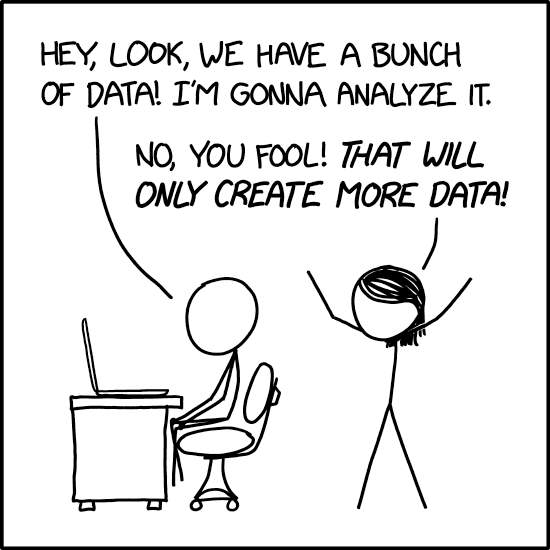
\includegraphics[width=0.35\textwidth]{img/data_trap.png}}
\end{figure}

% Math teachers
%\begin{figure}[h]
%	\centering
%	\href{https://xkcd.com/263/}{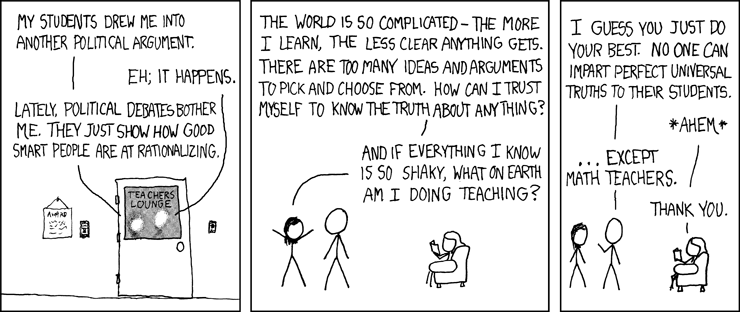
\includegraphics[width=0.9\textwidth]{img/certainty.png}}
%\end{figure}

% We ride!
%\begin{figure}[h]
%	\centering
%	\href{https://xkcd.com/1856/}{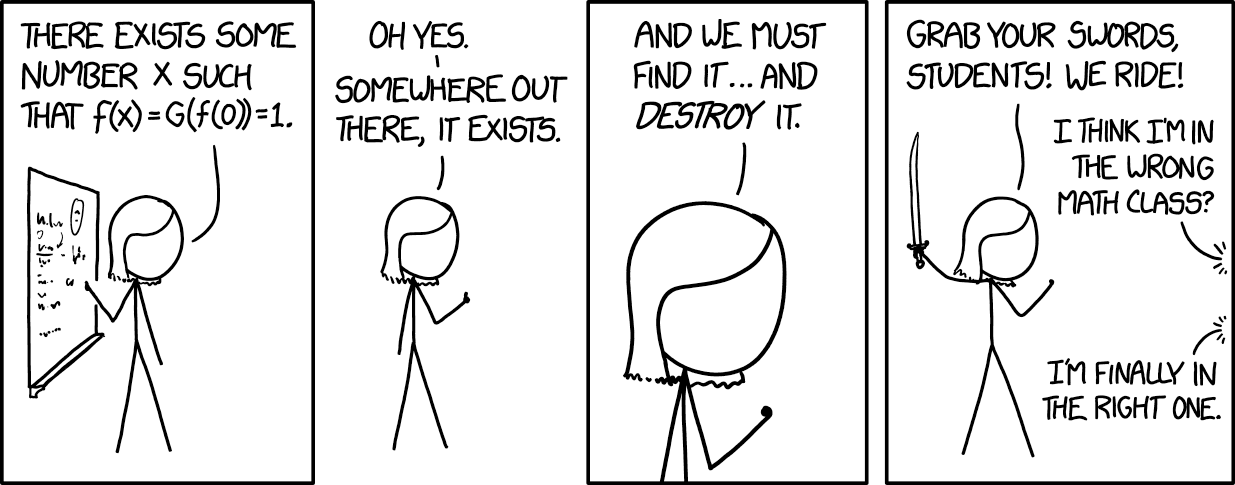
\includegraphics[width=0.8\textwidth]{img/existence_proof_2x.png}}
%\end{figure}

%\begin{quotation}
%	\noindent``\textit{You can't really know anything if you just remember isolated facts. If the facts don't hang together on a latticework of theory, you don't have them in a usable form. You've got to have models in your head.}''\\
%	\\
%	--Charlie Munger (investor, vice chairman of Berkshire Hathaway)
%\end{quotation}


\section*{Course Objectives}
%\vskip.15in
%\noindent\textbf{Course Objectives:}
By the end of this course, you will be able to:
\begin{itemize}
	\item Confidently work with data using the \texttt{R} programming language
	\item Create beautiful and informative data visualizations
	\item Organize your work so that it is transparent and reproducible
	\item Build basic statistical models and estimate their parameters from data
	\item Communicate the uncertainty around your estimates
	\item Identify research designs that credibly address three fundamental challenges of social science: measurement, causal inference, and sampling.
%	\item Explain the fundamental mathematics behind the statistical methods we use in political science (probability and inference, matrix algebra, and optimization).
%	\item Manipulate, wrangle, and clean datasets using the \texttt{R} programming language
%	\item Create beautiful data visualizations
%	\item Organize your work so that it is transparent and reproducible
%	\item Compute derivatives and solve systems of linear equations
%	\item Explain the properties of probability distributions and expected values
%	\item Perform hypothesis tests and fit models to data
\end{itemize}

%\section*{Course Structure}
%
%This will be a weird semester, and I expect that there will be more than the usual share of setbacks and hardships. Please don't hesitate to ask questions or reach out to me with your concerns.
%
%If you show any \href{https://www.google.com/search?q=covid-19+symptoms}{symptoms of COVID-19} or have been exposed to someone who tests positive for COVID-19, don't come to class. Obviously. I do not grade class attendance, and every piece of material that you need to succeed on assignments and tests will be made available online. I plan to simulcast our class sessions over Zoom and post recordings to the course website, and I will hold regular virtual office hours if you have questions that aren't covered in those places.
%
%When you come to class, please wear a mask. The University System of Georgia (USG) requires all faculty, students, and staff to wear appropriate face coverings while inside campus buildings. Reasonable accommodations may be made for those who are unable to wear a face covering for documented health reasons. Students seeking an accommodation related to face coverings should contact Disability Services at \href{https://drc.uga.edu/}{https://drc.uga.edu/}. For more information on the University of Georgia's coronavirus response, visit \href{https://coronavirus.uga.edu/}{https://coronavirus.uga.edu/}.
%
%Our classroom will have a limited capacity this semester (14 students), but that should be sufficient to have all enrolled students attend in person. Following the Thanksgiving break, all remaining class sessions will be held online.

\section*{Assignments \& Grading}

Each week I will assign 1-2 chapters of reading and a problem set, both due at noon the day of class. Feel free to consult your classmates with questions about the problem sets, but I expect you to submit your answers individually. \textbf{Resist the temptation to copy-paste your classmates' code.} You are much more likely to learn if you type your responses yourself. Each problem set will contain a \textbf{Bonus} problem that will require you to conduct some independent research beyond that week's reading. Problem sets will be graded pass/fail, where a passing grade indicates that you have correctly solved over 70\% of the problems. 

The semester will culminate with each student completing an independent research project. During the final two weeks, students will present an original analysis of a dataset of their choice. To meet expectations, the project should address in a satisfying way issues relating to measurement, causal inference, and sampling, and students should submit code and a codebook that allows others to replicate their analysis from the raw dataset. Within 48 hours of your presentation, I will provide you a list of revisions that I think would improve the research. Completing these revisions before the end of finals period is a requirement for earning an A- or A in the course. Students wishing to earn an A will---in addition to the presentation, code, and codebook---submit a final paper that includes an abstract, brief literature review, and discussion of their findings.

The final letter grade you earn for the semester will be determined based on the number of problem sets you complete that meet expectations, the number of bonus problems you successfully complete, and your performance on the final project. Consult the table below for the minimum requirements for each letter grade. To earn a given letter grade, you must complete the requirements for that grade and all the grades below it, and students must at least meet the requirements for a C to pass the course.\\\\
\begin{tabular}{|c|c|c|c|}
	\hline
	Letter Grade & Problem Sets & Bonus Problems & Final Project \\
	\hline
	A & 10 & 8 & Submit a final paper \\
	\hline
	A- & 9 & 5 & Complete requested revisions \\
	\hline
	B+ & 8 & 2 & Code successfully replicates \\
	\hline
	B & 7 & 0 & Provide code and codebook \\
	\hline
	C & 6 & 0 & Present final project \\
	\hline
\end{tabular} 

%\vskip.15in
%\noindent\textbf{Office Hours:}
\section*{Office Hours and Email Policy}
I will be available for students to drop in and chat every Monday, Wednesday, and Friday afternoon from 1:30-3pm. My office is Baldwin 304C. If you send me an email, please allow me 24 hours to respond. Like many professors, my inbox is pretty overloaded. Also, I have small children, so it's my policy to not check email after 5pm or on weekends. You should feel free to seek assistance from the senior graduate students staffing the SPIA Methods Helpdesk. You can email them questions at \href{mailto:spia-methods-help@uga.edu}{spia-methods-help@uga.edu}.


%\vskip.15in
%\noindent\textbf{Textbook:} %\footnotemark
\section*{Books}

Our readings will come from the two books listed below. The first book (DAFSS) must be purchased, but the second (R4DS) is freely available online.

%All of the assigned readings for this class will be available free online (including a few of the textbooks listed below). However, if you're the sort of person that prefers reading hard copies, I recommend these books!

\begin{itemize}

%\item \href{https://www.amazon.com/Quantitative-Social-Science-Introduction-tidyverse/dp/0691222274}{Imai, Kosuke, and Nora Webb Williams (2022). \textit{Quantitative Social Science: An Introduction in Tidyverse}. Princeton: Princeton University Press.}

\item \textbf{DAFSS:}  \href{https://press.princeton.edu/books/paperback/9780691199436/data-analysis-for-social-science}{Llaudet, Elena \& Imai, Kosuke (2022). \textit{Data Analysis for Social Science: A Friendly and Practical Introduction}. Princeton University Press.}

\item \textbf{R4DS:} \href{https://r4ds.hadley.nz/}{Wickham, H., Cetinkaya-Rundel, M., \& Grolemund, G., (2023). \textit{R For Data Science: Import, Tidy, Transform, Visualize, and Model Data, 2nd Edition}. O'Reilly Media, Inc.}

%\item \textbf{M\&S:}  \href{https://ebookcentral.proquest.com/lib/ugalib/detail.action?pq-origsite=primo&docID=1205618}{Moore, Will H., and David A. Siegel. 2013. \textit{A Mathematics Course for Political and Social Research}. Princeton, NJ: Princeton University Press.}

%\item \href{https://ebookcentral.proquest.com/lib/ugalib/reader.action?docID=3304559}{Strogatz, Steven H. 2012. \textit{The Joy of X: A Guided Tour of Math, from One to Infinity}. Boston: Houghton Mifflin Harcourt.}

%\item \href{https://theeffectbook.net/index.html.}{Huntington-Klein, Nick. 2021. \textit{The Effect: An Introduction to Research Design and Causality}. Chapman \& Hall CRC.}

%\item \href{https://www.amazon.com/Visual-Display-Quantitative-Information/dp/1930824130}{Tufte, Edward (2001). \textit{The Visual Display of Quantitative Information}}
%\item \href{https://socviz.co/}{Healy, Kieran (2018). \textit{Data Visualization: A Practical Introduction}. Princeton University Press.}




%\item \href{https://www.amazon.com/All-Statistics-Statistical-Inference-Springer/dp/1441923225}{Wasserman, L. (2013). \textit{All of Statistics: A Concise Course in Statistical Inference}. Springer Science \& Business Media.}
%\item \href{https://www.amazon.com/Mathematics-Economists-Carl-P-Simon/dp/0393957330}{Simon, C. P., \& Blume, L. (1994). \textit{Mathematics for Economists}. New York: Norton.}


\end{itemize}



\section*{Course Outline}

%Moltke the Elder writes that no battle plan survives first contact with the enemy. This is doubly true for syllabi. We may need to be flexible, and deviate from the plan if some topics require more or less attention, or we think of something completely unexpected that we want to do, and it takes up a few weeks. Caveats aside, here is what I have planned! %I've built in some Bonus Weeks towards the end of the semester that we can use for catch up. If everything goes according to plan, then we can cover extra topics during those weeks by popular demand.

\subsection*{\underline{PART 1: FUNDAMENTALS}}

%\begin{center}
%\begin{minipage}{6in}
%\begin{flushleft}
%Chapter 1 \dotfill ~$\approx$ 3 days \\
%{\color{darkgreen}{\Rectangle}} ~A little of probability theory and graph theory
\subsubsection*{Week 1: Getting Started}
\textit{Introductions, The Three Fundamental Problems of Scientific Inquiry}\\
\textbf{Reading Due}: None

\subsubsection*{Week 2: Writing Code}
\textit{Setting Up R and RStudio, Tidy Datasets, Variables, Basic Programming}\\
\textbf{Reading Due}: DAFSS Chapter 1

% ADVANCED TOPIC: Quarto

\subsubsection*{Week 3: Experiments}
\textit{Causal Inference, Potential Outcomes, Randomization, Estimation}\\
\textbf{Reading Due}: DAFSS Chapter 2

% ADVANCED TOPIC: ???

\subsubsection*{Week 4: Samples}
\textit{Descriptive Statistics, Representative Samples, Distributions, Basic Data Visualization}\\
\textbf{Reading Due}: DAFSS Chapter 3

% ADVANCED TOPIC: Non-representative samples (big data paradox)

\subsubsection*{Week 5: The Linear Model}
\textit{Regression, Logarithms, Prediction}\\
\textbf{Reading Due}: DAFSS Chapter 4

% ADVANCED TOPIC:

% This week we give the calculus lecture, just like normal, and the calculus problem set is due the week after.

%\subsubsection*{Week 7: Calculus}
%\textit{Derivatives, Optimization}\\
%\textbf{Reading Due}: M\&S Chapter 5%, Strogatz Chapter 17

\subsubsection*{Week 6: Causality}
\textit{Confounders, Multiple Regression, Internal and External Validity}\\
\textbf{Reading Due}: DAFSS Chapter 5

% This week you can give the Matrix Algebra lecture....if you want?? But there's no problem set for it, and Michael says he doesn't need it, so honestly, forget about it!

%\subsubsection*{Week 9: Matrix Algebra}
%\textit{Vectors, Matrices, Matrix Inverse, Ordinary Least Squares}\\
%\textbf{Reading Due}: M\&S Chapter 12 (ignore sections 12.3.6 and 12.3.7).

\subsubsection*{Week 7: Probability}
\textit{Sampling Distributions, Expected Value, Variance, Normal Distributions, Bernoulli Distributions, Central Limit Theorem, Law of Large Numbers}\\
\textbf{Reading Due}: DAFSS Chapter 6

\subsubsection*{Week 8: Uncertainty}
\textit{Hypothesis Testing, Confidence Intervals, Standard Errors, p-values,  Integrals, The Fundamental Theorem of Calculus}\\
\textbf{Reading Due}: DAFSS Chapter 7

% PART 2: Getting your hands dirty (applying the lessons from part 1 to real datasets / research projects)

\subsection*{\underline{PART 2: APPLICATIONS}}

\subsubsection*{Week 9: Visualize Your Data}
\textit{ggplot2, Exploration, Communication}\\
\textbf{Reading Due}: R4DS Chapters 1-2

\subsubsection*{Week 10: Transform Your Data}
\textit{Data Wrangling, Filtering, Summarizing, Code Style}\\
\textbf{Reading Due}: R4DS Chapter 3-4, 12

\subsubsection*{Week 11: Tidy Your Data}
\textit{Pivoting, Scripts, and Projects}\\
\textbf{Reading Due}: R4DS Chapter 5-6

\subsubsection*{Week 12: Import \& Export Your Data}
\textit{Pivoting, Scripts, and Projects}\\
\textbf{Reading Due}: R4DS Chapter 7-8

\subsubsection*{Week 13: Merge Your Data}
\textit{Keys, Joins, Fuzzy Record Linkage}\\
\textbf{Reading Due}: R4DS Chapter 19



%\subsubsection*{Week 3: Tools for Reproducible Research}
%\textit{Workflow, Documentation, File Structure, RMarkdown, \LaTeX, Zotero/Mendeley, \texttt{git} and GitHub}

%\subsubsection*{Week 5: Functions}
%\textit{Summation, Products, Logarithms, Exponentials, Writing Better Code, Flow Control}

%\subsubsection*{Week 7: Midterm}
%\textit{Mini-conference}

%\subsection*{PART 2: CAUSALITY}





%\subsubsection*{Week 10: Sneaking Through the Front Door}
%\textit{Experiments, Instrumental Variables, Regression Discontinuity}

%\subsection*{PART 3: UNCERTAINTY}




%\subsubsection*{Week 10: Matrix Algebra and OLS}
%\textit{Regression, Systems of Linear Equations, Independence, Matrix Multiplication, Matrix Inversion}
%
%\subsubsection*{Week 11: Models and Prediction}
%\textit{Fitting Models, Machine Learning, Overfitting, Cross-Validation, Regularization, Ensembles}

%\subsubsection*{Week 12: Bonus Week 1}
%Possible Topics: \textit{Causal Inference, Text-As-Data, Big Data, Machine Learning, Networks, Spatial Data, \texttt{blogdown, bookdown}, Advanced Reproducible Research}
%
%\subsubsection*{Week 13: Bonus Week 2}
%Possible Topics: \textit{Causal Inference, Text-As-Data, Big Data, Machine Learning, Networks, Spatial Data, \texttt{blogdown, bookdown}, Advanced Reproducible Research}
%
%\subsubsection*{Week 14: Bonus Week 3}
%Possible Topics: \textit{Causal Inference, Text-As-Data, Big Data, Machine Learning, Networks, Spatial Data, \texttt{blogdown, bookdown}, Advanced Reproducible Research}

\subsubsection*{Weeks 14-15: Wrap Up}
\textit{Review, Catch Up, Final Projects}


%\end{flushleft}
%\end{minipage}
%\end{center}

%\vskip.15in
%\noindent\textbf{Important Dates:}
%\begin{center} \begin{minipage}{3.8in}
%\begin{flushleft}
%Midterm \#1      \dotfill ~\={A}b\={a}n 16, 1393  \\
%Midterm \#2      \dotfill ~\={A}zar 21, 1393  \\
%%Project Deadline \dotfill ~Month Day \\
%Final Exam       \dotfill ~Dey 18, 1393  \\
%\end{flushleft}
%\end{minipage}
%\end{center}



\section*{Academic Honesty}
Remember that when you joined the University of Georgia community, you agreed to abide by a code of conduct outlined in the academic honesty policy called \href{https://honesty.uga.edu/Academic-Honesty-Policy/Introduction/}{\textit{A Culture of Honesty}}. You may consult other students with questions about problem sets, but I expect you to submit individual responses, and the final projects must be completed individually.

\section*{Mental Health and Wellness Resources}

\begin{itemize}
\item If you or someone you know needs assistance, you are encouraged to contact Student Care and Outreach in the Division of Student Affairs at 706-542-7774 or visit \href{https://sco.uga.edu}{https://sco.uga.edu}. They will help you navigate any difficult circumstances you may be facing by connecting you with the appropriate resources or services.
\item UGA has several resources for a student seeking \href{https://www.uhs.uga.edu/bewelluga/bewelluga}{mental health services} or \href{https://www.uhs.uga.edu/info/emergencies}{crisis support}.
\item If you need help managing stress anxiety, relationships, etc., please visit \href{https://www.uhs.uga.edu/bewelluga/bewelluga}{BeWellUGA} for a list of FREE workshops, classes, mentoring, and health coaching led by licensed clinicians and health educators in the University Health Center.
\item Additional resources can be accessed through the UGA App.
\end{itemize}



%%%%%% THE END
\end{document}